\section{Điều chỉnh trọng số tự động}
Phần này trình bày cách các trọng số $\omega_i$ được giới thiệu trong Phần 3.3 có thể tự động điều chỉnh khi sử dụng phương pháp thống kê từ các vòng lặp trước. Ý tưởng chung là theo dõi 1 điểm số đại diện cho độ hiệu quả của thuật toán trong các vòng lặp gần đây. Điểm số này càng cao thì thuật toán càng hiệu quả. Cả quá trình tìm kiếm được chia thành nhiều bước. 1 bước là 1 số vòng lặp của ALNS heuristic; ở đây tác giả chọn 1 bước là 100 vòng lặp. Điểm số heuristic được đặt bằng 0 khi bắt đầu mỗi bước và được tăng thêm $\sigma_1, \sigma_2, \sigma_3$ tùy các trường hợp ghi trong Bảng \ref{tab:1}.

Trong trường hợp $\sigma_1$ rõ ràng: Nếu một heuristic có thể tìm được một phương án tổng quan tốt nhất thì nó đã hoạt động tốt. Tương tự, Nếu heuristic  đã tìm thấy một phương án chưa từng được duyệt qua trước đó và được chấp nhận bởi điều kiện chấp nhận trong tìm kiếm ALNS thì heuristic đó thành công và thuật toán tìm kiếm lại tiếp tục. Có vẻ hợp lý để phân biệt giữa hai tình huống tương ứng với các tham số $\sigma_2$ và $\sigma_3$ vì chúng ta ưu tiên các heuristics có thể cải thiện phương án nhưng cũng không bỏ qua các heuristic có thể đa dạng hóa việc tìm kiếm, điều này liên quan đến $\sigma_3$. Cần nhấn mạnh rằng chúng ta chỉ cần quan tâm đến các phương án chưa được duyệt qua. Điều này khuyến khích heuristics có thể tìm ra những phần mới của không gian nghiệm. Chúng ta theo dõi các phương án đã được duyệt qua bằng các gán một khóa (\textit{hash key}) cho mỗi phương án và sắp xếp các khóa này trong một bảng băm (\textit{hash table}).

\begin{table}[caption={Kết quả tốt nhất, 200 địa điểm}, label=tab:1]
    % \resizebox{\textwidth}{!}{
        % \begin{tabularx}{\linewidth}{@{}>{\bfseries}l@{\hspace{.5em}}X@{}}
            \begin{tabular}{lp{10cm}}
            \hline
            Tham số     &   Mô tả \\
            \hline
            $\sigma_1$  &   Hoạt động xóa-chèn cuối cùng dẫn đến một phương án mới tốt nhất trong phạm vi toàn cục. \\
            $\sigma_2$  &   Thao tác xóa-chèn cuối cùng dẫn đến một phương án chưa được chấp nhận trước đó. Chi phí của phương án mới tốt hơn chi phí của phương án hiện tại. \\
            $\sigma_3$  &   Thao tác xóa-chèn cuối cùng dẫn đến một phương án chưa được chấp nhận trước đó. Chi phí của phương án mới tồi tệ hơn chi phí của phương án hiện tại, nhưng phương án đã được chấp nhận. \\
            \hline
        \end{tabular} \\
\end{table}

Trong mỗi vòng lặp, tác giả áp dụng 2 heuristic: xóa và chèn. Các điểm số cho cả 2 phương pháp heuristic được cập nhật cùng 1 lượng, vì ta không thể biết chắc chắn sự tốt lên của thuật toán là do phương thức xóa hay chèn.

Tại mỗi lần kết thúc 1 bước, ta tính toán lại trọng số mới sử dụng các điểm số cũ. Cho $\omega_{ij}$ là trọng số của heuristic \textit{i} được sử dụng tại bước \textit{j} với trọng số như trong công thức \ref{eq:20}. Trong bước đầu tiên, ta đánh trọng số các heuristic bằng nhau. Sau đó, khi bước \textit{j} kết thúc, ta tính toán trọng số cho tất cả heuristic \textit{i} để sử dụng cho bước thứ \textit{j} + 1 như sau:
\begin{equation}
    \omega_{i, j+1} = \omega_{ij}(1-r)+r\frac{\pi_i}{\theta_i}
\end{equation}
Trong đó, $\pi_i$ là điểm số của heuristic \textit{i} được nhận trong bước cuối cùng, $\theta_i$ là số lần ta cố gắng sử dụng heuristic \textit{i} trong bước thực hiện đó. \textit{Reaction factor - r} điều khiển cách trọng số điều chỉnh nhanh hay chậm, phản ứng với sự thay đổi của độ hiệu quả của thuật toán. Nếu \textit{r} = 0 thì ta không sử dụng điểm và các trọng số sẽ không đổi. Nếu \textit{r} = 1 thì điểm đánh giá được nhận trong lần thực hiện cuối cùng sẽ quyết định trọng số.

\begin{figure}[H] % places figure environment here   
    \centering % Centers Graphic
    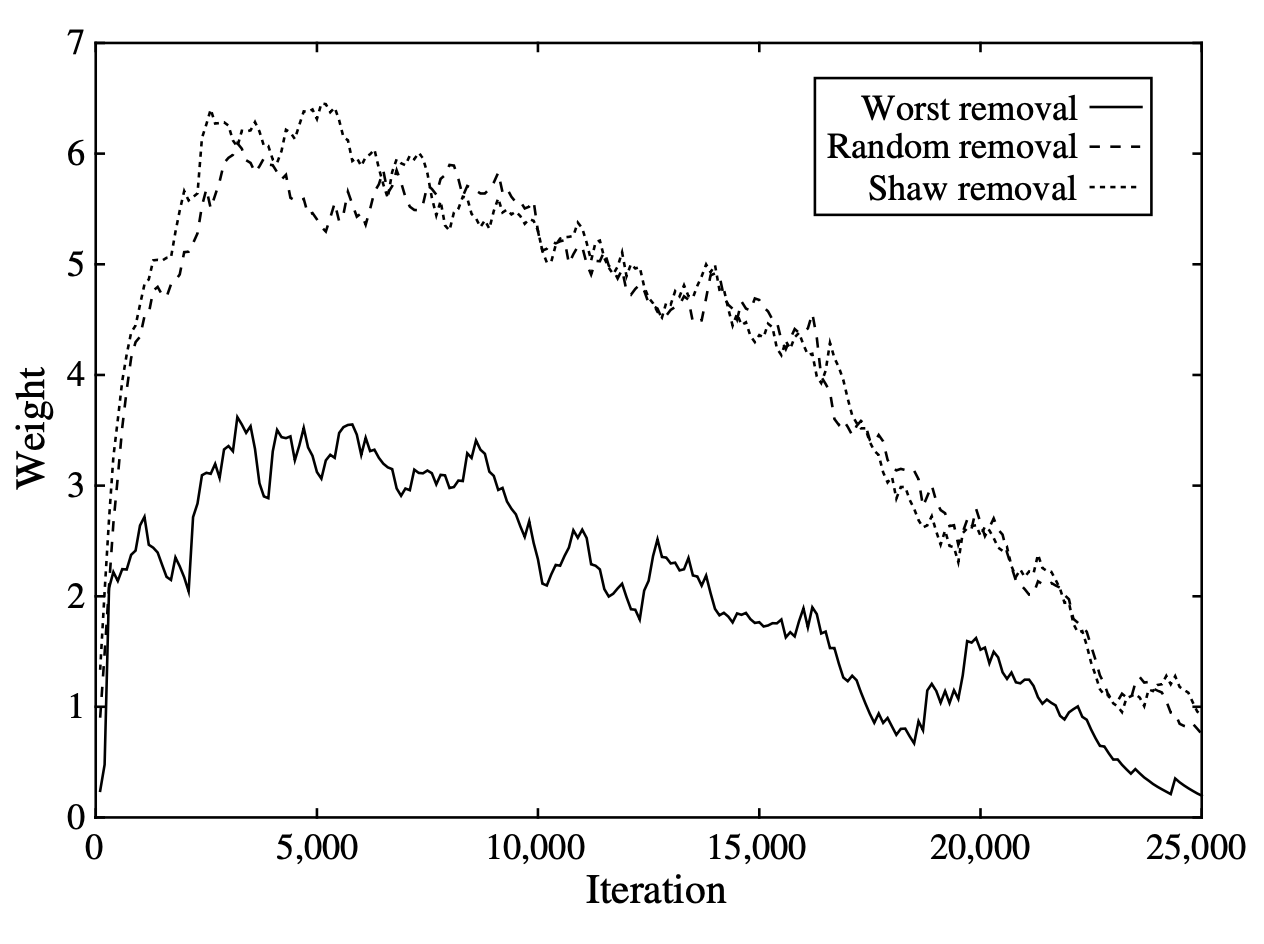
\includegraphics[width=0.8\textwidth]{figures/fig-1.png} 
    \caption{Đồ thị cho thấy cách các trọng số của 3 heuristic xóa biến đổi theo thời gian khi giải quyết 1 bài toán. Biểu đồ giảm dần vì các tiêu chí mô phỏng chỉ chấp nhận các nước di tốt, do đó heuristic khó đạt điểm cao} % Creates caption underneath graph
    \label{fig:fg_01}
\end{figure}
\textit{Ghi chú: trục $x$ là số vòng lặp và trục $y$ là trọng số. Đồ thị minh hoạ cho một bài toán cụ thể, phương pháp xoá ngẫu nhiên và phương pháp xoá Shaw thể hiện gần như nhau, trong khi phương pháp xoá tệ nhất thể hiện kém nhất. Thế nên, phương pháp xoá tệ nhất không được sử dụng thường xuyên như 2 phương pháp còn lại.}
